\chapter{Các hệ thống và công nghệ liên quan}

% Nhiều hệ thống danh tiếng và công nghệ liên quan đã được phát triển nhằm phục vụ các mục tiêu khác nhau như đánh giá sản phẩm, xác thực hành vi, hoặc hỗ trợ ra quyết định trong môi trường trực tuyến. 
% Bài báo ``Reputation systems: A survey and taxonomy'' \cite{reputation-systems-survey-taxonomy} đã xây dựng một hệ thống phân loại cho các hệ thống danh tiếng.
% Cấp độ đầu tiên trong hệ thống phân loại này dùng để phân biệt giữa các hệ thống danh tiếng được thiết kế tường minh (explicit) và các hệ thống danh tiếng ngầm định (implicit).
% như thu thập dữ liệu (Collection), 
% tổng hợp (Aggregation), tính ngữ cảnh (Context), hay khả năng tương tác giữa các hệ thống (Interoperability). 
% Dưới đây là một số hệ thống và công nghệ tiêu biểu mà chúng tôi sẽ trình bày trong chương này

\section{ReGreT}

\textbf{ReGreT} \cite{regret-reputation-system} là một mô hình đánh giá uy tín trong xã hội nhiều tác nhân (multi-agent society), được xây dựng nhằm mô phỏng cách con người hình thành và sử dụng danh tiếng trong các tương tác xã hội.
Mô hình này mở rộng so với các mô hình trước bằng cách đưa ra ba chiều chính (dimension) của uy tín: chiều cá nhân, chiều xã hội, và chiều bản thể học (ontological).

\subsection{Chiều cá nhân}

Đây là mức độ cơ bản nhất của uy tín, dựa trên trải nghiệm trực tiếp giữa hai tác nhân. Khi hai tác nhân tương tác, mỗi bên ghi nhận \textit{kết quả} (outcomes) từ tương tác đó, bao gồm những gì đã được thỏa thuận và những gì thực sự xảy ra.
Dựa vào những kết quả này, mỗi tác nhân hình thành \textit{ấn tượng cá nhân} (impressions), từ đó tính ra \textit{uy tín chủ quan} (subjective reputation). Bên cạnh đó, cũng sẽ một
\textit{độ tin cậy} (reliability) đối với uy tín chủ quan này. Những ấn tượng gần thời điểm hiện tại hơn sẽ được ưu tiên cao hơn thông qua hàm trọng số thời gian.

Từ đó, ReGreT định nghĩa cách tính uy tín trực tiếp của một tác nhân $a$ đối với tác nhân $b$ (chiều cá nhân) như sau:
\[R_{a \rightarrow b}(subject)\]

\subsection{Chiều xã hội}

ReGreT mô hình hóa hiện tượng phổ biến trong xã hội con người: một cá nhân mang theo uy tín của nhóm mà họ thuộc về.
Nếu không có đủ thông tin trực tiếp, ta có thể dựa vào uy tín nhóm để ước lượng hành vi của một tác nhân.
Tương tự như cách một cá nhân có thể bị ảnh hưởng bởi uy tín của nhóm mà mình thuộc về, bản thân cá nhân đó cũng sẽ dựa vào \textit{trải nghiệm} (experiences)
của những người trong chính nhóm của mình để bổ sung và củng cố hiểu biết cá nhân về một thực thể.
Nói cách khác, những gì mà các thành viên trong nhóm từng trải qua với một thực thể cụ thể (hoặc với nhóm của thực thể đó) sẽ góp phần định hình
và làm phong phú thêm nhận định của mỗi thành viên trong nhóm.

Do đó, để tính giá trị uy tín của mình đối với một tác nhân theo chiều xã hội, ReGreT mở rộng thêm ba nguồn thông tin mới. Bên cạnh tương tác trực tiếp với chính tác nhân, giờ đây phải xem xét thêm
tương tác với các thành viên trong nhóm mà tác nhân đó thuộc về, thông tin mà nhóm của mình đối với tác nhân đó, và cuối cùng là thông tin mà nhóm của mình đối với nhóm của tác nhân đó.

\subsubsection{Trải nghiệm cá nhân}

Giả sử ta tính giá trị uy tín của một tác nhân $a$ thuộc về nhóm $\mathcal{A}$ đối với tác nhân $b$ thuộc về nhóm $\mathcal{B}$.
Đầu tiên, ta đã biết uy tín trực tiếp giữa hai tác nhân như sau:
\[R_{a \rightarrow b}(subject)\]

Tiếp theo, sự tương tác của $a$ đối với các thành viên khác của nhóm $\mathcal{B}$ được biểu diễn như sau:
\[R_{a \rightarrow \mathcal{B}}(subject)=\sum_{b_i \in \mathcal{B}} \omega^{ab_i} \cdot R_{a \rightarrow b_i}(subject)\]
trong đó, $\sum_{b_i \in \mathcal{B}} \omega^{ab_i} = 1$. Vì đang trong trường hợp uy tín chủ quan, chúng ta cần
phương thức để thể thiện độ tin cậy của uy tín này:
\[RL_{a \rightarrow \mathcal{B}}(subject)=\sum_{b_i \in \mathcal{B}} \omega^{ab_i} \cdot RL_{a \rightarrow b_i}(subject)\]

\subsubsection{Trải nghiệm nhóm}

Một khi đã có được trải nghiệm của cá nhân $a$, ta sẽ xem xét đến trải nghiệm của nhóm $\mathcal{A}$ đối với tác nhân $b$ và cả nhóm $\mathcal{B}$.

Đầu tiên, ta tính uy tín chủ quan của nhóm $\mathcal{A}$ đối với tác nhân $b$ cùng với độ tin cậy của uy tín như sau:
\[R_{\mathcal{A} \rightarrow b}(subject)=\sum_{a_i \in \mathcal{A}} \omega^{a_ib} \cdot R_{a_i \rightarrow b}(subject)\]
\[RL_{\mathcal{A} \rightarrow b}(subject)=\sum_{a_i \in \mathcal{A}} \omega^{a_ib} \cdot RL_{a_i \rightarrow b}(subject)\]
trong đó, $\sum_{a_i \in \mathcal{A}} \omega^{a_ib} = 1$.

Tương tự, để biết được uy tín của nhóm $\mathcal{A}$ đối với nhóm $\mathcal{B}$, ta tính như sau:
\[R_{\mathcal{A} \rightarrow \mathcal{B}}(subject)=\sum_{a_i \in \mathcal{A}} \omega^{a_i\mathcal{B}} \cdot R_{a_i \rightarrow \mathcal{B}}(subject)\]
\[RL_{\mathcal{A} \rightarrow \mathcal{B}}(subject)=\sum_{a_i \in \mathcal{A}} \omega^{a_i\mathcal{B}} \cdot RL_{a_i \rightarrow \mathcal{B}}(subject)\]
trong đó, $\sum_{a_i \in \mathcal{A}} \omega^{a_i\mathcal{B}} = 1$.

\subsubsection{Tổng hợp tất cả thông tin lại với nhau}

Cuối cùng, ReGreT định nghĩa cách tính uy tín của tác nhân $a$ đối với tác nhân $b$ theo chiều xã hội như sau:
\begin{align*}
  SR_{a \rightarrow b}(subject) =\  & \xi_{ab} \cdot R_{a \rightarrow b}(subject) +                                       \\
                                    & \xi_{a\mathcal{B}} \cdot R_{a \rightarrow \mathcal{B}}(subject) +                   \\
                                    & \xi_{\mathcal{A}b} \cdot R_{\mathcal{A} \rightarrow b}(subject) +                   \\
                                    & \xi_{\mathcal{A}\mathcal{B}} \cdot R_{\mathcal{A} \rightarrow \mathcal{B}}(subject)
\end{align*}
\begin{align*}
  SRL_{a \rightarrow b}(subject) =\  & \xi_{ab} \cdot RL_{a \rightarrow b}(subject) +                                       \\
                                     & \xi_{a\mathcal{B}} \cdot RL_{a \rightarrow \mathcal{B}}(subject) +                   \\
                                     & \xi_{\mathcal{A}b} \cdot RL_{\mathcal{A} \rightarrow b}(subject) +                   \\
                                     & \xi_{\mathcal{A}\mathcal{B}} \cdot RL_{\mathcal{A} \rightarrow \mathcal{B}}(subject)
\end{align*}
trong đó, $\xi_{ab} + \xi_{a\mathcal{B}} + \xi_{\mathcal{A}b} + \xi_{\mathcal{A}\mathcal{B}} = 1$.

\subsection{Chiều bản thể học}

Trong hai chiều cá nhân và xã hội, mỗi lần đánh giá uy tín chỉ tập trung vào một khía cạnh đơn lẻ. Tuy nhiên, trong thực tế,
các khía cạnh này thường liên quan đến nhau và cần được kết hợp cùng \textit{trọng số} của từng khía cạnh lại để hình thành một khái niệm uy tín phức tạp hơn --
đó chính là mục tiêu của \textbf{chiều bản thể học}.

Ở chiều này, mô hình ReGreT sử dụng cấu trúc đồ thị để mô tả mối quan hệ giữa các khía cạnh khác nhau của uy tín.
Ví dụ, \textit{một người bán hàng tốt} (good seller) có thể bao gồm các yếu tố: giao hàng nhanh, giá cả hợp lý, và chất lượng sản phẩm cao,
ta có cấu trúc đồ thị bản thể như hình \ref{fig:good-seller-ontological-structure} để mô hình hóa mối quan hệ giữa các khía cạnh trong ví dụ này.

\begin{figure}[H]
  \centering
  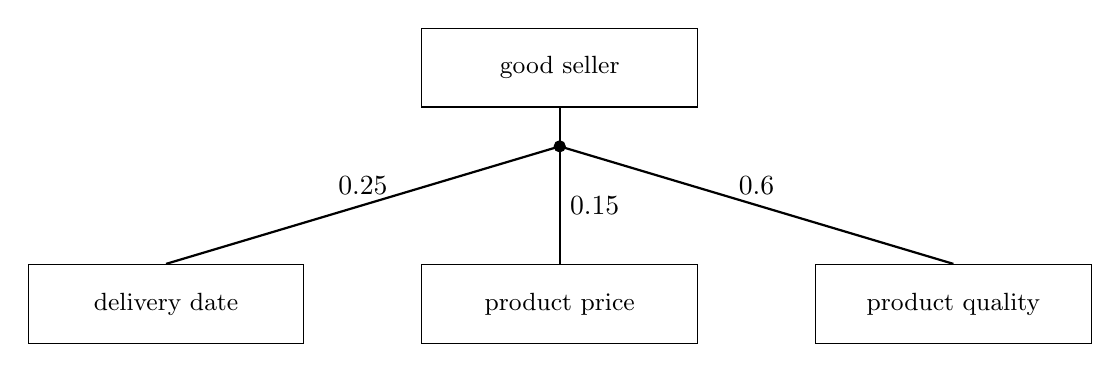
\begin{tikzpicture}
    \node[draw, rectangle, minimum width=3.5cm, minimum height=1cm, font=\small] at (5,0) (goodseller) {good seller};
    \node[draw, rectangle, minimum width=3.5cm, minimum height=1cm, font=\small] at (0,-3) (deliverydate) {delivery date};
    \node[draw, rectangle, minimum width=3.5cm, minimum height=1cm, font=\small] at (5,-3) (productprize) {product price};
    \node[draw, rectangle, minimum width=3.5cm, minimum height=1cm, font=\small] at (10,-3) (productquality) {product quality};

    \filldraw[black] (5,-1) circle (2pt);

    \draw[thick] (goodseller.south) -- (5,-1);
    \draw[thick] (deliverydate.north) -- (5,-1) node[midway, above] {0.25};
    \draw[thick] (productprize.north) -- (5,-1) node[midway, right] {0.15};
    \draw[thick] (productquality.north) -- (5,-1) node[midway, above] {0.6};
  \end{tikzpicture}
  \caption{Cấu trúc đồ thị bản thể cho ``một người bán hàng tốt''}
  \label{fig:good-seller-ontological-structure}
\end{figure}

Vì vậy, khi muốn tính một uy tín phức hợp theo chiều bản thể học, một tác nhân cần tính uy tín của từng khía cạnh liên quan.
Mỗi khía cạnh này có thể lại là một nút trong một đồ thị con, nơi nó cũng được cấu thành từ các khía cạnh nhỏ hơn nữa.

Đối với những nút cuối cùng trong đồ thị (các khía cạnh cơ bản nhất của hành vi, gọi là \textit{atomic aspect}),
thì uy tín của chúng được tính dựa trên chiều cá nhân và chiều xã hội.

Sau khi có điểm uy tín cho từng nút con, điểm uy tín của một nút bất kỳ $i$ trong đồ thị bản thể sẽ được tính bằng cách kết hợp
các giá trị của các nút con của nó theo một công thức:
\[OR_{a \rightarrow b}(i) = \sum_{j \in children(i)} w_{ij} \cdot OR_{a \rightarrow b}(j)\]
\[ORL_{a \rightarrow b}(i) = \sum_{j \in children(i)} w_{ij} \cdot ORL_{a \rightarrow b}(j)\]
trong đó, $OR_{a \rightarrow b}(j) = SR_{a \rightarrow b}(j)$ khi $j$ là một khía cạnh cơ bản.

Đối với ví dụ ở hình \ref{fig:good-seller-ontological-structure}, ta có thể tính giá trị uy tín của $b$ (người bán hàng tốt)
từ góc nhìn của $a$ bằng công thức:
\begin{align*}
  OR_{a \rightarrow b}(good\ seller) =\  & 0.25 \cdot SR_{a \rightarrow b}(delivery\ date) + \\
                                        & 0.15 \cdot SR_{a \rightarrow b}(product\ price) + \\
                                        & 0.6 \cdot SR_{a \rightarrow b}(product\ quality)
\end{align*}